
\documentclass[12pt]{article}
% Standard ams packages
\usepackage{amsmath, amssymb, amsthm, graphicx}
\usepackage{tikz}
% Edit margins
\usepackage[letterpaper, margin=1in, left=0.8in]{geometry}
\setcounter{section}{-1}
% Resume enumeration after a break
\usepackage{enumitem}
\makeatletter
\def\verbatim@nolig@list{\do\`\do\<\do\>\do\'\do\-}% no comma
\makeatother
%\pagenumbering{gobble}

% Define macros
\global\long\def\dom{\mathop\mathrm{dom}\nolimits}   % domain
\global\long\def\Ker{\mathop\mathrm{Ker}\nolimits} % kernel
\global\long\def\Im{\mathop\mathrm{Im}\nolimits} % image
\global\long\def\C{\mathbb{C}}                       % complex
\global\long\def\R{\mathbb{R}}                       % reals
\global\long\def\Q{\mathbb{Q}}                       % rationals
\global\long\def\Z{\mathbb{Z}}                       % integers
\global\long\def\N{\mathbb{N}}                      % naturals

\def\div{\, \big| \,} % divides
\def\inv{^{-1}} % inverse
\def\tr{\text{Trace}} % trace
\def\GL{\text{GL}} % general linear
\def\SL{\text{SL}} % special linear
\def\char{\text{char}} % characteristic

% Generator of a group
\newcommand{\gen}[1]{\langle #1 \rangle}
\renewcommand{\qedsymbol}{\(\blacksquare\)}

\theoremstyle{plain}
\newtheorem{corollary}{Corollary}
\newtheorem{lemma}{Lemma}
\newtheorem{example}{Example}
\newtheorem{observation}{Observation}
\newtheorem{proposition}{Proposition}
\newtheorem{theorem}{Theorem}
\newtheorem{axiom}{Axiom}
\newtheorem{question}{Question}

\theoremstyle{definition}
\newtheorem{definition}{Definition}

\theoremstyle{remark}
\newtheorem{remark}{Remark}

% Quick permutation group notation (3 elements)
\newenvironment{permutation3}
{
\left(\begin{tabular}{ccc}
}
{
\end{tabular}\right)
}

% Quick permutation group notation (4 elements)
\newenvironment{permutation4}
{
\left(\begin{tabular}{cccc}
}
{
\end{tabular}\right)
}

% Quick permutation group notation (5 elements)
\newenvironment{permutation5}
{
\left(\begin{tabular}{ccccc}
}
{
\end{tabular}\right)
}

% Quick permutation group notation (6 elements)
\newenvironment{permutation6}
{
\left(\begin{tabular}{cccccc}
}
{
\end{tabular}\right)
}

% Quick permutation group notation (7 elements)
\newenvironment{permutation7}
{
\left(\begin{tabular}{ccccccc}
}
{
\end{tabular}\right)
}

\title{Number Theory Fundamentals}
\author{Bahattin Yildiz }
\date{}
\begin{document}

\maketitle
\section{Preliminaries on Notation and Sets}
In this section we will go over some of the notations and basic concepts that we will be talking about throughout the rest of the material. 
We start with a naive definition of a set:
\begin{definition}
A ``set" is an unordered collection of objects, called elements, where there are no repetitions. 
\end{definition}

We will usually denote sets with letters such as $A, B, C$, etc. $a\in A$ will mean that ``$a$ is an element of $A$", or that ``$a$ is in $A$", or that ``$a$ belongs to $A$", any one of which can be used. 

{\bf Standard Description of Sets:} For an ambient domain $A$ and a property $P$ defined on $A$, we will use notations such as 
$$\{x\in A| P(x)\: is\: true\}$$
to describe the set of all elements in $A$ that satisfy the property $P$. 
Before moving onto some examples of this notation, let us recall some special sets that we will be dealing with:
\begin{align*}
&\N = \{1, 2, 3, \dots, \},\:\:\:\:\textrm{Positive Integers or Natural Numbers},\\
&\Z = \{\dots, -2, -1, 0, 1, 2, 3, \dots, \},\:\:\:\:\textrm{Integers},\\ 
& \Q = \{a/b| a,b \in \Z, b\neq 0\}, \:\:\:\:\textrm{Rationals},\\
&\R, \:\:\:\:\: \:\:\:\:\textrm{Real Numbers},\\
& \C = \{a+bi| a,b \in \R\} \:\:\:\:\textrm{Complex Numbers}.
\end{align*}

\begin{example}
\begin{enumerate}
    \item $\{a\in \Z| \frac{a}{2}\in \Z\}$ is another way of describing the even integers.
    \item $\{a\in \Z|a>0\}$ is another way of describing $\N$. 
    \item $\{a\in \Z|a>0, a\equiv 1\pmod{3}\}$, $\{a\in \N|a\equiv 1\pmod{3}\}$, $\{1+3k|k=0,1,2, \dots \}$, $\{1,4,7,10, \dots \}$
    are all equivalent notations for the set of positive integers that are $1$ mod $3$. 
\end{enumerate}
\end{example}

\section{The Division Algorithm} 

The division algorithm is attributed to Euclid, and hence is sometimes called the ``Euclidean Division Algorithm". The following is the most general statement of the theorem:
\begin{theorem} {\bf $($The Division Algorithm$)$ }
Let $a, b \in \Z$ be integers with $b\neq 0$. Then there is a unique pair $q,r$ of integers such that 
$$a=bq+r, \:\:\:\:\:\:\: 0\leq r<|b|.$$
\end{theorem}

\begin{theorem} {\bf $($The Division Algorithm for Positive integers$)$ }
Let $a, b$ be nonnegative integers with $b>0$. Then there is a unique pair $q,r$ of integers such that 
$$a=bq+r, \:\:\:\:\:\:\: 0\leq r<b.$$
\end{theorem}

\hrule

\bigskip
\noindent

\begin{remark}
    \begin{enumerate}
        \item There are many different versions of the Division algorithm that can be proved using the same idea. For example:
        \\
        Given $a,b\in \Z$ such that $b\neq 0$, there are unique integers $q,r$ such that $a=bq+r$, with $-\frac{|b|}{2} < r\leq \frac{|b|}{2}$. 
    \item More examples like the previous one can be given. The main idea is that the remainder can be put in an interval of length $|b|$.
    \end{enumerate}
\end{remark}

\begin{example}
    Let us do a division activity, using Theorem 6. In the following, for given $a, b$ determine what the $q$ and $r$ should be upon dividing $a$ by $b$.  

\begin{itemize}
    \item $a=-3,\: b=2$. $-3=2\cdot (-2)+1$, so the quotient is $-2$ and the remainder is 1.
    \item $a=12,\: b=-5$.  $12 = (-5)\cdot (-2)+2$, so the remainder is $2$ and the quotient is $-2$.
\end{itemize}
\end{example}

\bigskip
\hrule

\bigskip 
\noindent
Let us now see some consequences of the division algorithm. 
\begin{corollary}
    \begin{itemize}
        \item If $m$ is any positive integer greater than 1, then the remainder of any number upon dividing by $m$ is $0, 1, 2, \dots m-1$. 
        \item Every integer is of the form $2k$ or $2k+1$.
        \item Every integer is of the form $3k$, $3k+1$ or $3k+2$.
        \item Every integer is of the form $4k$, $4k+1$, $4k+2$ or $4k+3$
.    \end{itemize}
\end{corollary}

\bigskip
\noindent
\begin{example}
\begin{itemize}
    \item $a(a^2+2)$ is a multiple of 3 for every integer $a$. 
    \item $a^2$ is of the form $4k$ or $4k+1$ for all integers $a$.
\end{itemize}
    
\end{example}


\bigskip
\hrule

	\section{Divisibility}
Divisibility follows from the previous section very naturally as we will be considering the special case of the remainder in the division algorithm to be 0.

\begin{definition}
    Let $a,b \in \Z$ with $b\neq 0$. If $a=bq$ for some $q\in \Z$ (i.e., the remainder is 0) then we say ``$b$ divides $a$", or ``$a$ is a multiple of $b$", or ``$b$ is a divisor of $a$" of ``$a$ is divisible by $b$", which are all equivalent. In mathematical notation we denote this by ``$b|a$".
\end{definition}
\begin{example}
Here are some quick examples following from the definition. 
\begin{itemize}
    \item $3|3$,  \:\:\:\: $5|10$, \:\:\:\: $-2|4$, \:\:\:\: $2|6$, \:\:\:\: $5|(-15)$.
    \item $a|0$ if $a\neq 0$.
    \item $a|a$ if $a\neq 0$.
    \item $1|a$ and $-1|a$ for all $a\in \Z$.
\end{itemize}
\end{example}


\bigskip
\hrule

\bigskip
\noindent
We will now give a major theorem that will give us all the ``algebra" of divisibility:

\begin{theorem} $($ The Algebra of Divisibility $)$
For integers $a, b, c, d$ the following hold:
\begin{enumerate}
    \item $a|0$ $(a\neq 0)$, $1|a$, $a|a$ $(a\neq 0)$.
    \item $a|1$ if and only if $a=\pm 1$.
    \item If $a|b$ and $c|d$, then $ac|bd$.
    \item If $a|b$ and $b|c$, then $a|c$. 
    \item $a|b$ and $b|a$ if and only if $a=\pm b$
    \item If $a|b$ and $b\neq 0$, then $|a|\leq |b|$. 
    \item If $a|b$ and $a|c$, then $a|(bx+cy)$ for all $x,y\in \Z$. 
\end{enumerate}
\end{theorem}

\bigskip
\hrule

\section{GCD}

The main application of divisibility theorems come in the form of GCD, which is defined as the ``greatest common divisor". 
\begin{definition}
Let $a, b$ be non-negative integers, not both zero. We say $GCD(a,b)=d$ for some positive integer $d$ if 
\begin{enumerate}
    \item $d|a$ and $d|b$, (so $d$ is a common divisor, the ``C") and
    \item If $e$ is a positive number such that $e|a$ and $e|b$, then $e\leq d$ (so $d$ is the greatest among divisors, the ``G").  
\end{enumerate}
\end{definition}

\begin{example} Here are some examples following directly from the definition:
\begin{enumerate}
    \item If $a\in \N$, then $GCD(a,0)=a$.
    \item If $a\in \N$, then $GCD(a,a)=a$.
    \item If $a\in \N$, then $GCD(1,a) =1$.
    \item If $a,b \in \N$ such that $a|b$, then $GCD(a,b)=a$. 
\end{enumerate}
\end{example}

\begin{definition}
If $GCD(a,b)=1$, then $a$ and $b$ are called to be relatively prime.
\end{definition}

\begin{example}
$6$ and $11$ are relatively prime. Similarly, 15 an 32 are relatively prime. 
\end{example}

\begin{theorem} {\bf $($B\'ezout$)$}
If $a, b$ are non-negative integers, not both zero, then there exists $x, y \in \Z$ such that 
$$d=GCD(a,b) = ax+by.$$
\end{theorem}

\bigskip
\begin{remark}
Note that $x, y$ can be negative numbers and they do not have to be unique. For example, if $a=3$ and $b=7$, then we can write 
$$GCD(3,7) = 1 = (-2)\cdot 3+1\cdot 7 = 5\cdot 3+(-2)\cdot 7.$$
\end{remark}

\bigskip
\noindent
Theorem 4 has a special case in which the assertion becomes a double-implications:

\begin{theorem}
If $a, b\in \N$, then $GCD(a,b) = 1$ if and only if there exists $x, y$ such that $ax+by = 1$. 
\end{theorem}

There are two very important corollaries of Theorem 5. 

\begin{corollary} $($ Euclid's Lemma$)$
If $a|bc$ and $GCD(a,b)=1$, then $a|c$
\end{corollary}

\begin{corollary} $($Euclid's Second Lemma$)$
Suppose $GCD(a,b)=1$. If $a|c$ and $b|c$, then we must have $ab|c$.
\end{corollary}

\bigskip
\hrule

\section{The Euclidean Algorithm}
\begin{itemize}
    \item It calculates the GCD without the G, C, or D. (not the method used in middle school or high school). Does not use prime numbers at all.
    \item Very efficient and fast
    \item Not only does it calculate $GCD(a,b)$, but also helps us find $x, y\in \Z$ such that $GCD(a,b)=ax+by$. 
\end{itemize}

\hrule

\bigskip
\noindent
The whole algorithm depends on the following lemma:
\begin{lemma}
If $a$ and $b$ are two positive integers, then $GCD(a,b)=GCD(a-kb,b) = GCD(a, b-ma)$ for all integers $k$ and $m$.
\end{lemma} 
\begin{remark}
$k$ and $m$ can be positive as well as negative integers. So, essentially, what the lemma is saying is that, for example,  
$$GCD(a,b) = GCD(a-2b, b) = GCD(a, b+3a)=GCD(a,b-5a)  = GCD(a+b,b) = \dots $$
\end{remark}

\bigskip
\noindent
{\bf How can we use the lemma to calculate GCD?}
Here are a couple of early examples of how we can use the Lemma before we see the algorithm:
\begin{itemize}
    \item $GCD(28,12) =GCD(4.7,4.3)=4GCD(7,3)=4.$
\end{itemize}

\bigskip
\hrule

\bigskip
\noindent The whole algorithm depends on the following special case of Lemma 1: \\
Let $a, b$ be positive integers such that $a>b$. By applying the division algorithm, we get $a=bq+r$, where $0\leq r<b$. Then we have 
$$GCD(a,b) = GCD(a-bq, b) = GCD(r,b) = GCD(b,r).$$
So the idea is that we are replacing $GCD(a,b)$ by $GCD(b,r)$ so that $b<a$ and $r<b$. \\
So, here is the formal Euclidean algorithm:

\bigskip
\noindent
{\bf The Euclidean Algorithm:} Suppose $a$ and $b$ are two positive integers with $a>b$. 
\begin{verbatim}
    If b|a then GCD = b. Else 
    with a=bq+r GCD(a,b) = GCD(b,r).
\end{verbatim} 

\begin{example}
Let us apply the algorithm to find $(92,28)$ and the coefficients $x,y$ such that $(92,28)=92x+28y$. 

We do a sequence of division algorithms:
\begin{align*}
    92&=3\cdot 28+8 \\
    28&=3\cdot 8+4\\
    8&=2\cdot 4.
\end{align*}
So $GCD(92,28)=4$. To find the coefficients $x, y$ in the Extended algorithm, we start with the last line and go backwards: 
\begin{align*}
    4 & = 28-3\cdot 8 \\
     & = 28-3(92-3\cdot 28) = (-3)\cdot 92+10\cdot 28. 
\end{align*}
\end{example}

\bigskip
The algorithm can be used to prove the following observation aboout GCDs:
\begin{theorem}\label{factorout}
If $k\in \N$ and $a, b$ are positive integers, then $(ka, kb) = k(a,b)$.
\end{theorem}

\bigskip
This result has an immediate corollary:
\begin{corollary}
If $(a,b)=d$, then $(\frac{a}{d}, \frac{b}{d}) =1$. 
\end{corollary}

\bigskip
\noindent {\bf GCD of more than two numbers:} Suppose $a_1, a_2, \dots, a_n$ are $n$ positive integers. Then we say 
$$(a_1, a_2, \dots, a_n) = d$$ if 
\begin{itemize}
    \item $d|a_1$, $d|a_2$, $\dots$, $d|a_n$, and 
    \item If $e|a_1$, $e|a_2$, $\dots$, $e|a_n$, then $e\leq d$ (or $e|d$). 
\end{itemize}

\begin{remark}
Following the same arguments used in the proof of Theorem 9 (B\'ezout's), it can be shown that there exists integers $x_1, x_2, \dots, x_n$ such that 
$$(a_1, a_2, \dots, a_n) = a_1x_1+a_2x_2+\dots +a_nx_n.$$
\end{remark}

\bigskip
\noindent
Another approach to calculating the GCD of more than two elements can be accomplished by a recursive argument that is given in the following theorem:
\begin{theorem}
If $a, b, c$ are positive integers, then we have
$$GCD(a,b,c) = GCD(GCD(a,b),c) = GCD(a, GCD(b,c)) = GCD(b,GCD(a,c)).$$
\end{theorem}

\bigskip
\begin{example}
$GCD(12, 20, 60) = GCD(12,GCD(20,60)) = GCD(12,20)=GCD(3\cdot 4, 5\cdot 4) = 4\cdot GCD(3,5)=4.$
\end{example}

\subsection{LCM}
\begin{definition}$($ LCM$)$
Let $a$ and $b$ positive integers. We say the {\it lowest common multiple} of $a$ and $b$ is $m$, i.e., $LCM(a,b) = m$ if 
\begin{itemize}
    \item $a|m$ and $b|m$ and
    \item If $a|c$ and $b|c$, then $m\leq c$. 
\end{itemize}
\end{definition}

\begin{remark}
If $(a,b)=1$, what is $LCM(a,b)=ab$.
\end{remark}

\begin{theorem}\label{gcdlcm}
If $(a,b) = d$, then $LCM(a,b) = \frac{ab}{d}$.
In other words, $(a,b)\cdot LCM(a,b) = ab$.
\end{theorem}

\begin{example} Let us find $LCM(12,30)$:
$$LCM(12, 30) = \frac{12 \cdot 30}{GCD(12,30)} = \frac{12\cdot 30}{6} = 60.$$
\end{example}
The following corollary follows from Theorem \ref{factorout} and Theorem \ref{gcdlcm}:
\begin{corollary}
If $k$ is a positive integer, then  $LCM(ka,kb)=kLCM(a,b)$.
\end{corollary}

\bigskip
\hrule

\section{Prime Numbers}
\bigskip
\noindent
We first start with the definition of a prime number:
\begin{definition}
A positive integer $p>1$ is called a {\it prime number} if $a|p$ implies $a=1$ or $a=p$. In other words, a prime number has only $1$ and itself as positive divisors.  
\end{definition}
We should also include the definition of a {\it composite number} at this point:
\begin{definition}
A positive integer $m>1$ is called {\it composite} if it is not prime. In other words, $m>1$ is said to be composite if there exists $a,b $ such that $1<a, b <m$ and $m=ab$.
\end{definition}
\begin{remark}
$1$ is neither a prime number nor a composite number. 1 is a unit, and as such does not belong to any of the two categories. 
\end{remark}

\begin{example}
The first few primes can be listed as 
$$2, 3, 5, 7, 11, 13, 17, 19, 23, 29, 31, 37, 41, 43, 47, 53, 59, 61, 67, 71, 73, \dots $$
\end{example}
\begin{remark}
2 is the only even prime number. Every prime greater than 2 has to be odd. 
\end{remark}

\begin{observation}
By the definition of prime numbers, we can observe that any integer $>p$ that is divisible by $p$ has to be composite. Thus we have 
\begin{itemize}
    \item any prime number greater than 3 has to be of the form $3k+1$ or $3k+2$
    \item any prime number greater than $3$ has to be of the form $4k+1$ or $4k+3$
    \item any prime number greater than $3$ has to be of the form $6k+1$ or $6k+5$. (why?)
\end{itemize}
\end{observation}
\hrule

\begin{observation}
There is no known closed form function that gives all the prime numbers. For example, $x^2+x+41$ is prime for all values of $x=0, 1, \dots, 39$. But, there certainly are values of $x$ for which this function is not prime. (Can you think of some such values?)
\end{observation}
\hrule

\bigskip
\noindent

The following lemma is a useful property of prime numbers and does not require proof, since it follows directly from the definition:
\begin{lemma}
If $p$ is a prime number and $a$ is any integer, then 
$$GCD(a,p) = \left \{ \begin{array}{ll}
p & \textrm{if $p|a$ }\\
1 & \textrm {if $p\nmid a$}
\end{array}\right.$$
\end{lemma}

\hrule

\bigskip
\noindent
This lemma leads to the following variant of Euclid's Lemma, which is instrumental in proving the Fundamental Theorem of Arithmetic:
\begin{lemma}$($Euclid's Lemma: Primes$)$ Let $p$ be a prime number. Then $p|ab$ implies $p|a$ or $p|b$.
\end{lemma}

\bigskip
\noindent
\begin{remark}
\begin{itemize}
\item A most common mistake in Number Theory is to apply the lemma with a non-prime number. The assumption that $p$ is a prime is essential for the lemma. For example, $6|4\cdot 3$, but $6\nmid 4$ and $6\nmid 3$.  
\item Using Mathematical Induction, the lemma can easily be extended to more than two numbers. I.e., if $p$ is prime, then 
$p|a_1a_2\dots a_k$ implies $p|a_i$ for some $i$. 
\end{itemize}
\end{remark}
\hrule

\bigskip
\noindent
\begin{theorem}$($ Fundamental Theorem of Arithmetic: FTA$)$ Every integer $n>2$ can be written as a product of prime numbers uniquely. In other words, if $$n=p_1p_2\dots p_k = q_1q_2\dots q_m,$$ with $p_i$ and $q_j$ prime numbers, then $k=m$ and (after a reordering of terms if necessary), we have $p_i=q_i$. 
\end{theorem}

\bigskip
\noindent
Thus, given any $n>1$, we can write $n=p_1^{\alpha_1}p_2^{\alpha_2} \dots p_k^{\alpha_k}$, where $p_1, p_2, \dots, p_k$ are prime numbers and $\alpha_i$ are positive integers. This is also called the ``prime factorization" of $n$.

\bigskip
\noindent
{\bf Some Consequences of the FTA}
\\
\begin{enumerate}
    \item {\bf The number of positive divisors}: Let $n=p_1^{\alpha_1}p_2^{\alpha_2} \dots p_k^{\alpha_k}$. Then we can find a formula for the number of positive divisors of $n$, which we denote by $\tau(n)$ from this factorization:
    $$\tau(n)=(1+\alpha_1)(1+\alpha_2)\dots (1+\alpha_k).$$
    \item Let $n$ be any positive integer. Then we can write $n=2^kA$, where $k\geq 0$ and $A$ is odd. 
    \item {\bf GCD \& LCM} The factorization gives us a more familiar (albeit not practical) way of calculating the GCD and LCM of two numbers:
\\
Suppose $m,n \geq 0$ and assume that 
$$m=p_1^{\alpha_1}p_2^{\alpha_2} \dots p_k^{\alpha_k},$$
$$n=p_1^{\beta_1}p_2^{\beta_2} \dots p_k^{\beta_k}$$
where $\alpha_i, \beta_i \geq 0$. (why did we let them be $\geq 0$?)
Then we can write 
$$GCD(m,n) = p_1^{\min(\alpha_1, \beta_1)}\cdot p_2^{\min(\alpha_2, \beta_2)} \cdot \dots \cdot p_k^{\min(\alpha_k, \beta_k)}$$
and 
$$LCM(m,n) = p_1^{\max(\alpha_1, \beta_1)}\cdot p_2^{\max(\alpha_2, \beta_2)} \cdot \dots \cdot p_k^{\max(\alpha_k, \beta_k)}.$$
\end{enumerate}

\subsection{The Sieve of Eratosthenes} 
Suppose we want to determine whether $659$ is prime or not. How can we answer this? The Sieve of Eratosthenes gives us the first example of what is known as a {\bf Primality test}, The sieve depends on the following theorem:
\begin{theorem} $($Eratosthenes $)$
If $n>1$ is composite, then there exists a prime number $p$ such that $p\leq \sqrt{n}$ and $p|n$. 
\end{theorem}

\bigskip
\noindent
What makes this theorem really useful is the following corollary, which is just the contrapositive equivalent of the theorem:
\begin{corollary}
If $n>1$ is NOT divisible by any of the primes $\leq \sqrt{n}$, then $n$ must be prime. 
\end{corollary}

\bigskip
\subsection{Bertrand's Theorem}
In 1840s, Bertrand conjectured something about prime numbers, which he could not prove. The conjecture was proved later by Chebyshev, which is why I would like to label the theorem as Bertrand-Chebyshev:
\begin{theorem}$($ Bertrand-Chebyshev$)$
For any $n>1$, there is at least one prime number between $n$ and $2n$. 
\end{theorem}

\bigskip
\begin{corollary}\begin{enumerate}
    \item If $p_n$ denotes the $n$th prime number, then $p_n \leq 2^n$.
    \item There are at least $\lfloor \log_2n\rfloor $ primes less than $n$. 
\end{enumerate}
\end{corollary}

\bigskip
\noindent
{\bf The Actual Prime Number Theorem:} Let $\Pi(n)$ denote the number of prime numbers less than $n$. Then $\Pi(n) \simeq \frac{n}{\log n}$ for large $n$, where $\log$ is the natural log.

\bigskip
\hrule

\section{Congruences}
We will focus on two main topics in this chapter: the definition and algebra of congruences and linear congruences.
\subsection{The Definition and Algebra of Congruences}
\begin{definition}
Let $n>1$ be a positive number. For integers $a,b$ we say $a\equiv b \pmod{n}$ (``$a$ is congruent to $b$ modulo $n$") if $n|a-b$, or equivalently $a-b=nk$ for some integer $k$. 
\end{definition}

\bigskip
\begin{observation}
By division algorithm, if $n>1$ is any integer and $a$ is some integer, then $a=qn+r$, where $0\leq r <n$. In this case, we have $a\equiv r \pmod{n}$. Thus for any integer $n>1$, an integer $a$ is always congruent to one of $0, 1, 2, \dots, n-1$ modulo $n$. 
For example if $n=3$, then we have 
$$18\equiv 243\equiv -6 \equiv -45 \equiv 0 \pmod{3},$$
$$20\equiv 122\equiv -4 \equiv -40 \equiv 2 \pmod{3},$$
$$10\equiv 109\equiv -5 \equiv -35 \equiv 1 \pmod{3}.$$
\end{observation}
\hrule

\bigskip
\noindent
We are now ready to state the main theorem regarding congruences:
\begin{theorem}$($ Algebra of Congruences$)$
Let $n>1$ be an integer and $a, b, c, d$ be any integers. Then 
\begin{enumerate}
    \item $a\equiv a \pmod{n}$.
    \item If $a\equiv b \pmod{n}$, then $b\equiv a \pmod{n}$.
    \item If $a\equiv b \pmod{n}$ and $b\equiv c \pmod{n}$, then $a\equiv c \pmod{n}$.
    \item If $a\equiv b \pmod{n}$ and $c\equiv d \pmod{n}$, then $a+c\equiv b+d \pmod{n}$ and $ac\equiv bd \pmod{n}$. 
    \item If $a\equiv b \pmod{n}$, then $a+c\equiv b+c \pmod{n}$ and $ac\equiv bc \pmod{n}$ for all $c\in \Z$. 
    \item If $a\equiv b \pmod{n}$, then $a^k \equiv b^k \pmod{n}$ for all positive integers $k$. 
\end{enumerate}
\end{theorem}

\begin{remark}
We would like to observe that properties (1)-(3) tell us that the congruence relation is an equivalence relation.
\end{remark}

\section{Fermat's Little Theorem}
We will first start with the concept of complete residue classes:
\subsection{Complete Sets of Residue Classes (CSRC)}
Recall that by division algorithm, for an integer $n>1$, any integer is congruent modulo to $n$ to one of the numbers in $\{0,1,2, \dots, n-1\}$. Such a set is an example of a CSRC. 
\begin{definition}
A set $\{a_1, a_2, \dots, a_n\}$ is called a CSRC modulo $n$ if every integer is congruent to exactly one of the $a_i$s. Equivalently, such a set will be a CSRC if they are all incongruent modulo $n$, i.e., $a_i\not \equiv a_j \pmod{n}$ whenever $i\neq j$. 
\end{definition}
\begin{example}
Let us write down some examples of CSRC modulo $4$ and modulo $5$:
\\
$\{17,-22, 0, 11\} $ is a complete set of residue classes modulo $4$ since they reduce to $\{1,2,0,3\}$ modulo $4$.
\\
$\{2, 25, -17, 171, 4\} $ is a complete set of residue classes modulo 5 since they reduce to $\{2,0,3,1,4\}$ modulo 5.
\end{example}

\subsection{Cancellation Property}
Recall, from the previous chapter, that if $a\equiv b \pmod{n}$, then $ac\equiv bc \pmod{n}$ for all $c\in \Z$. But is the converse true? In other words, if we have $ac\equiv bc \pmod{n}$, then can we cancel out $c$ and say $a\equiv b \pmod{n}$?

\bigskip
\noindent
The following theorem tells us exactly how the cancellation property works and it forms a basis for many important subsequent results:
\begin{theorem} $($Cancellation Property$)$
If $ac\equiv bc \pmod{n}$, then $a\equiv b \pmod{\frac{n}{d}}$, where $d=GCD(c,n)$. 
\end{theorem}

\bigskip
\noindent
The theorem has many profound corollaries, some of which follow directly:
\begin{corollary}
If $GCD(c,n)=1$, then $ac\equiv bc \pmod{n}$ implies $a\equiv b \pmod{n}$.
\end{corollary}
\begin{corollary}
Let $p$ be a prime and suppose $ax\equiv ay \pmod{p}$ and that $p\nmid a$. Then $x\equiv y \pmod{p}$.
\end{corollary}
\begin{corollary}\label{CSRC}
Suppose $n>1$ is a positive integer and $a\in \Z$ satisfies $GCD(a,n)=1$. If $\{x_1, x_2, \dots, x_n\}$ is a CSRC modulo $n$, then $\{ax_1, ax_2, \dots, ax_n\}$ is also a CSRC modulo $n$.  
\end{corollary}
\begin{example}
Let us illustrate this on an example modulo $8$:
\\
If we multiply $\{0,1,2,3,4,5,6,7\}$ by $3$ then we get 
$$\{0,3,6,9,12,15,18,21\} \equiv \{0,3,6,1,4,7,2,5\} \pmod{8}.$$
\end{example}

\subsection{Two Main Results Following Corollary \ref{CSRC}}
\begin{theorem}$($Multiplicative Inverse Theorem $)$ \label{MultInv}
Let $n>1$ be an integer. If $GCD(a,n)=1$, then $a$ has a {\it unique} {\bf multiplicative inverse} modulo $n$, i.e., there exists a unique $x$ modulo $n$ such that 
$$ax \equiv 1 \pmod{n}.$$
\end{theorem}

\bigskip
\begin{remark}
There is another way of finding the multiplicative inverse of $a$ modulo $n$. Can you remember a way? For example, can we find the multiplicative inverse of 233 modulo 1079. Indeed, the Extended Euclidean Algorithm can be used to find 
$$233\cdot 389-1079\cdot 84=1.$$
Now, if we reduce this modulo $1079$, we see that $233^{-1}=389$ modulo $1079$. 
\end{remark}

\bigskip
\noindent
The next theorem is a very well-known congruence theorem, also known as Fermat's Little Theorem:
\begin{theorem}$($Fermat's Little Theorem$)$\label{FLiT}
Let $p$ be a prime number and $a\in \Z$ be such that $p\nmid a$. Then $$a^{p-1}\equiv 1 \pmod{p}.$$
\end{theorem}
 \bigskip
 \begin{example}
 Let us apply the theorem for some congruences:
 \begin{itemize}
     \item Let us reduce $(1723)^{103}$ modulo 5.
We first start with $1723\equiv 3\pmod{5}$. Using FLT, we have $3^4\equiv 1\pmod{5}$. Then we can write $3^{103}=(3^4)^{25}\cdot 3^3 \equiv 3^3\equiv 2\pmod{5}$. 
     \item Let us reduce $(1723)^{103}$ modulo 11. Similarly, $1723\equiv 7 \pmod{11}$ so we get $7^{103}$. Using FLT, we have $7^{10}\equiv 1 \pmod{11}$. So we get $7^{103} = (7^{10})^{10}\cdot 7^3 \equiv 7^3 = 49\cdot 7 \equiv 5\cdot 7 \equiv 2\pmod{11}.$
      \end{itemize}
 \end{example}

\bigskip
\hrule
\section{Linear Congruences}
The equation $ax=b$ has a unique solution in real numbers as long as $a\neq 0$.\\
What if $a,b$ are integers and we are looking for solutions in $\Z$?
Then the equation has a solution if and only if $a|b$. \\
But now the question is about the linear congruence: $ax\equiv b \pmod{n}$, where $n>1$ is a positive integer and $a, b$ are integer coefficients. A solution of this congruence is $x$ modulo $n$ that satisfies this congruence. Two solutions $x_1, x_2$ are different iff $x_1\not \equiv x_2 \pmod{n}$.

\bigskip
\noindent
{\bf Questions} We will try to answer the following questions regarding linear congruences:
\begin{enumerate}
    \item When does $ax\equiv b \pmod{n}$ have solutions?
    \item If solutions exist, how many incgonruent solutions are there?
    \item Can we describe all solutions?
\end{enumerate}

\bigskip
\noindent
We will answer all these questions by a theorem, but before that let us see some particular examples:
\begin{example}
Consider the following congruences: \\
$2x\equiv 4 \pmod{8}$. This has two solutions: $2, 6$. \\ 
$4x\equiv 0 \pmod{8}$. This has four solutions: $0,2,4,6$. \\
$2x\equiv 3 \pmod{8}$. This has no solutions since $2x=3+8k$ implies even=odd. \\
$3x\equiv 5 \pmod{8}$. This has a unique solution. $x=7$.  
\end{example}

\bigskip
\begin{theorem}
The congruence $ax\equiv b \pmod{n}$ has solutions if and only if $(a,n)|b$. Moreover, if $d=(a,n)$, then the congruence has exactly $d$ incongruent solutions. 
\end{theorem}

\bigskip
\noindent
Before going on to specific examples, it is worth observing the following corollary:
\begin{corollary}
If $GCD(a,n)=1$, then $ax\equiv b \pmod{n}$ has a unique solution for all $b \in \Z$.
\end{corollary}

\bigskip
\begin{example}
Let us find all the solutions of the congruence 
$$9x\equiv 21 \pmod{30}.$$
We first cancel $3$, which leads to $3x\equiv 7 \pmod{10}$. Multiplying both sides by $7$, we get $x\equiv 9 \pmod{10}$. Then the three solutions are given by $9, 9+10, 9+20$. 
\end{example}

\bigskip
\hrule
\section{The Chinese Remainder Theorem}
Chinese Remainder Theorem is about solving a system of linear congruences. We will see the theorem, some examples and an information security application of it. 
\begin{theorem} $($Chinese Remainder Thoerem: CRT $)$ \label{CRT} Ler $n_1, n_2, \dots, n_k$ be positive integers $>1$ so that $(n_i,n_j)=1$ for all $i, j$ with $i\neq j$. Then the system of congruence 
\begin{align*}
    x &\equiv a_1 \pmod{n_1} \\
    x &\equiv a_2 \pmod{n_2} \\
    &.\\
    &.\\
    &.\\
    x &\equiv a_k \pmod{n_k} 
\end{align*}
has a unique solution modulo $n_1n_2\dots n_k$.
\end{theorem}
\begin{proof}
We will give the proof here since it entails a constructive solution for the CRT. 

We first define $N=n_1n_2\dots n_k$ and let $N_i=N/n_i$, i.e., the product of all the $n_j$s except $n_i$. By the assumption in the theorem, we have $GCD(N_i, n_i)=1$. Then $N_i$ has a multiplicative inverse modulo $n_i$, let us denote it by $N_i^{-1}$. Then 
$$x=a_1N_1N_1^{-1}+a_2N_2N_2^{-1}+\dots +a_kN_kN_k^{-1}$$
is a solution of the system of equivalences. For example, reducing $x$ modulo $n_1$, we notice that $N_2, N_3, \dots, N_k$ are all divisible by $n_1$ so we get 
$$x\equiv a_1N_1N_1^{-1} \equiv a_1 \pmod{n_1}. $$ Similarly other congruences are checked. 
\end{proof}
\hrule
\medskip

The following picture describes how CRT works:

\bigskip

\begin{tikzpicture}
\tikzstyle{point2}=[ball color=green, circle, draw=black, inner sep=0.1cm]
 
    \node[rectangle,draw,  minimum width = 2cm, 
    minimum height = 2cm] (r1) at (0,0) {$\pmod{m_1}$};
    
\node [below] (P1) at (r1.south) {$a_1$};

 \node[rectangle,draw,  minimum width = 2cm, 
    minimum height = 2cm] (r2) at (4,0) {$\pmod{m_2}$};
\node [below] (P2) at (r2.south) {$a_2$};

\filldraw[black] (6,0) circle (2pt); 
 
\filldraw[black] (8,0) circle (2pt); 

\filldraw[black] (10,0) circle (2pt);
 \node[rectangle,draw,  minimum width = 2cm, 
    minimum height = 2cm] (rk) at (12,0) {$\pmod{m_k}$};

\node [below](Pk) at (rk.south) {$a_k$};

\node (X) at (6,-4) [point2] {$x$};
\draw (X)--(P1);
\draw (X)--(P2);
\draw (X)--(Pk);
\end{tikzpicture}
\bigskip
\begin{example}
Let us find the unique solution of the following system, using CRT:
\begin{align*}
    x &\equiv 2 \pmod{3} \\
    x &\equiv 1 \pmod{5} \\
    x &\equiv 3 \pmod{7}.
    \end{align*}
$N_1=5\cdot 7=35$, $N_2=3\cdot 7=21$, $N_3=3\cdot 5=15$.
$N_1^{-1}=2$ modulo $35$, $N_2^{-1}=1$ modulo $5$ and $N_3^{-1} = 1$ modulo $7$. Then 
$$x = 2\cdot 35\cdot 2+1\cdot 21\cdot 1+3\cdot 15\cdot 1 = 206 \equiv 101 \pmod{105}.$$

\bigskip

\begin{tikzpicture}
\tikzstyle{point2}=[ball color=green, circle, draw=black, inner sep=0.1cm]
 
    \node[rectangle,draw,  minimum width = 3cm, 
    minimum height = 3cm] (r1) at (0,0) {$\pmod{3}$};
    
\node [below] (P1) at (r1.south) {$2$};

 \node[rectangle,draw,  minimum width = 3cm, 
    minimum height = 3cm] (r2) at (6,0) {$\pmod{5}$};
\node [below] (P2) at (r2.south) {$1$};
 \node[rectangle,draw,  minimum width = 3cm, 
    minimum height = 3cm] (rk) at (12,0) {$\pmod{7}$};

\node [below](Pk) at (rk.south) {$3$};

\node (X) at (6,-4) [point2] {$101$};
\draw (X)--(P1);
\draw (X)--(P2);
\draw (X)--(Pk);
\end{tikzpicture}


\end{example}

\bigskip
\begin{example}
We can use CRT to find the multiplicative inverse of 233 modulo 880. Writing $880=16\cdot 5\cdot 11$ we can reduce the modular equation $233x\equiv 1 \pmod{880}$ to the congruence system:
\begin{align*}
    233x &\equiv 1 \pmod{16} \\
    233x &\equiv 1 \pmod{5} \\
    233x &\equiv 1 \pmod{11}.
    \end{align*}
\end{example}

\bigskip
\hrule
\section{A special quadratic congruence} 
We start with the following lemma:
\begin{lemma}
If $p$ is a prime number greater than $2$, then the congruence $x^2\equiv 1 \pmod{p}$ has exactly two solutions: $x\equiv 1$ and $x\equiv -1 \pmod{p}$. 
\end{lemma}
\begin{remark}
The lemma is not true for non-prime congruences. For example, $x^2\equiv 1 \pmod{8}$ has $4$ solutions, $x=1, 3, 5, 7$. 
\end{remark}
\begin{corollary}
If $p$ is an odd prime number, then for $1\leq x \leq p-1$, we have $x=x^{-1}$ mod $p$ if and only if $x\equiv 1$ or $x\equiv -1 \pmod{p}$.
\end{corollary}
\begin{proof}
This follows from observing $x\equiv x^{-1} \pmod{p}$ if and only if $x^2\equiv 1 \pmod{p}$
\end{proof}
\hrule



\bigskip
\begin{theorem}
Let $p$ be an odd prime. If $x^2\equiv -1 \pmod{p}$ has a solution, then $p$ must be of the form $4k+1$.
\end{theorem}

\bigskip
\begin{corollary}
If $p$ is of the form $4k+3$, then $x^2\equiv -1 \pmod{p}$ does not have solutions.
\end{corollary}

\begin{theorem}
If $p$ is a prime of the form $4k+1$, then $x^2\equiv -1 \pmod{p}$ has two solutions given by $x=\pm\left( \frac{p-1}{2}\right )!$
\end{theorem}

\bigskip
\hrule

\section{Euler's $\phi$-function}
Euler is one of the most prominent and productive mathematicians of all times. He has many contributions to many different fields. One of his most well-known contributions is in the field of congruences, for which we need the definition of the Euler $\phi$-function:
\begin{definition}
For an integer $n\geq 1$, the Euler $\phi$ of $n$ is defined to be the number of positive integers $\leq n$ that are relatively prime to $n$. In mathematical language:
$$\phi(n):= |\{1\leq a \leq n| GCD(a,n)=1\}|.$$
\end{definition}
\begin{example}
Let us find $\phi$ of numbers from 1 to 10 just by definition:
$\phi(1)=1=\phi(2)$, $\phi(3)=\phi(4)=2$, $\phi(5)=4$, $\phi(6)=2$, $\phi(7)=6$, $\phi(8)=4$, $\phi(9)=6$, $\phi(10)=4$.
\end{example}
\hrule

\bigskip
\noindent
We have several observations based on the definition and properties of GCD:
\begin{enumerate}
    \item If $p$ is a prime, then $\phi(p) = p-1$ since $1,2, \dots, p-1$ are all relatively prime to $p$.
 \item Moreover, for $n\geq 2$, $\phi(n) = n-1$ if and only if $n$ is prime.
 \item If $n>2$, then $\phi(n)$ is always even. (Why?)
 Because $GCD(a,n)=GCD(n-a,n)$.
 \item If $p$ is prime and $n$ is a positive integer, then 
 $\phi(p^n)=p^n-p^{n-1} = p^{n-1}(p-1)$. That is because, the numbers that are not relatively prime are given by $p\cdot 1, p\cdot 2, \dots, p\cdot (p^{n-1}-1)$.
\end{enumerate}
\hrule

\bigskip
\noindent
In order to find a general formula for $\phi(n)$, we need an important property of the Euler $\phi$-function. We will build up towards this major property by going through some minor ones:
\begin{lemma}
For positive integers $a, m, n$ we have 
$$GCD(a,mn)=1 \Leftrightarrow GCD(a,m)=GCD(a,n)=1.$$
\end{lemma}

\bigskip
\noindent
\begin{lemma}
If $a\equiv b \pmod{m}$, then $GCD(a,m)=GCD(b,m)$.
\end{lemma}
\begin{proof}
This simply follows from the fact that $a\equiv b \pmod{m}$ implies $a=b+mk$ for some integer $k$ and hence 
$GCD(a,m) = GCD(b+mk,m) = GCD(b+mk-mk,m) = GCD(b,m)$. 
\end{proof}

\bigskip
\noindent
\begin{lemma}
Suppose $(n,m)=1$ and $k\in \Z$ is any integer. Then
$$\{n\cdot 0+k, n\cdot 1+k, n\cdot 2+k, \dots, n\cdot(m-1)+k\}$$
is a CSRC modulo $m$.
\end{lemma}

\bigskip
\noindent
We are now ready to state a very important property of the Euler $\phi$-function.
\begin{theorem}\label{phi}
If $(m,n) = 1$, then $\phi(mn)=\phi(m)\phi(n)$. (In other words, the Euler $\phi$-function is a multiplicative number theoretic function.)
\end{theorem}

\subsection{The formula for the $\phi$-function}
A major application of Theorem \ref{phi} is that we can use it to find a formula for the Euler $\phi$-function.
\begin{theorem}\label{phi-formula}
If $n$ is a positive integer with a prime factorization of  $n=p_1^{\alpha_1}p_2^{\alpha_2} \dots p_k^{\alpha_k}$, where $\alpha_i\geq 1$, then 
$$\phi(n) = n\left(1-\frac{1}{p_1}\right)\left(1-\frac{1}{p_2}\right)\dots \left(1-\frac{1}{p_k}\right).$$
\end{theorem}
\begin{proof}
This follows because by Theorem \ref{phi} we have 
$$\phi(p_1^{\alpha_1}p_2^{\alpha_2} \dots p_k^{\alpha_k}) = \phi(p_1^{\alpha_1})\phi(p_2^{\alpha_2}) \dots \phi(p_k^{\alpha_k})$$
\end{proof}

\begin{remark}
The computational advantage of the above formula is that we do not need to find the full factorization of $n$ to find $\phi(n)$, instead we just need to find the prime divisors of $n$.  
\end{remark}

\bigskip
\noindent
\begin{example}
Let us find $\phi(360)$ using the theorem. Note that $2,3, 5$ are the prime divisors of $360$ and so 
$$\phi(360) = 360\left (1-\frac{1}{2}\right ) \left (1-\frac{1}{3}\right )\left (1-\frac{1}{5}\right ) = 360\cdot \frac{1\cdot 2\cdot 4}{30}=96.$$
\end{example}

\bigskip
\hrule
\section{Euler's Congruence Theorem}
Recall that, by Fermat's Little Theorem, we have $a^{p-1} \equiv \pmod{p}$, for all primes $p$ and integers $a$ such that $p\nmid a$. 
\\
The goal in this chapter is to extend this result to non-prime modulus.
For, this we will need the concept of ``complete set of reduced residue classes" (CSRRC):
\begin{definition}
Let $m>1$ be a positive integer. A CSRRC modulo $m$ is a set of $\phi(m)$ numbers, each of which is congruent to exactly one element in the set 
$$\Z_m^{\times}:= \{1\leq a\leq m| GCD(a,m)=1\}.$$
\end{definition}

\bigskip
\begin{example}
Let us see some examples of these CSRRCs:
$$\Z_5^{\times} = \{1,2,3,4\}, \:\:\:\:\Z_6^{\times} = \{1,5\}, \:\:\: \Z_8^{\times} = \{1,3,5,7\}.$$
\end{example}

\bigskip
\noindent
The following lemma is the final tool we need to prove Euler's congruence theorem:
\begin{lemma}
If $m>1$ is an integer and $a$ is an integer such that $(a,m)=1$, then 
$$a\Z_m^{\times} \equiv \Z_m^{\times} \pmod{m}.$$
In other words, if $\{x_1, x_2, \dots, x_{\phi(m)}\}$ is a CSRRC mod $m$, then so is
$\{ax_1, ax_2, \dots, ax_{\phi(m)}\}$.
\end{lemma}

\bigskip
\noindent
\begin{theorem}$($Euler's Congruence Theorem $)$ \label{EulerCong}
Let $m>1$ and $a$ be any integer such that $(a,m) =1$. Then we have
$$a^{\phi(m)} \equiv 1 \pmod{m}.$$
\end{theorem}

\bigskip
\noindent
Before going on to examples, we should note that Fermat's Little Theorem is an immediate corollary:
\begin{corollary}
If $p$ is prime and $p\nmid a$, then $a^{p-1} \equiv 1\pmod{p}$.
\end{corollary}

\begin{example}
Let us find $5^{261}$ modulo 18: Since $\phi(18)=6$ we have 
$5^{6} \equiv 1 \pmod{18}$ and so we have 
$$5^{261} = (5^6)^{43} \cdot 5^3 \equiv 5^3 =25\cdot 5 \equiv 35 \equiv 17 \pmod{18}.$$
\end{example}

\bigskip
\noindent
\begin{corollary}
If $GCD(a,m)=1$, then $a^{\phi(m)-1}$ is the multiplicative inverse of $a$ modulo $m$.
\end{corollary}

\begin{corollary}
Suppose $GCD(a,m)=1$. If $n\equiv d \pmod{\phi(m)}$, then 
$$a^n \equiv a^d \pmod{m}.$$
\end{corollary}

\bigskip
\hrule

\section{Cryptographic Applications of Euler's Congruence: 3-Pass Protocol and RSA}
We will talk about two main applications, which mainly use congruences, and in particular Euler's Congruence:
\subsection{The 3-Pass Protocol}
Supopose Alice and Bob are living far away from each other and Alice wants to send a secret tucked in safely in a locked box to Bob. The problem is only Alice has the key to the lock, and she CANNOT send the key to Bob because then Eve the eavesdropper will intercept the key and will be able to access the secret? The 3-pass protocol allows this transfer to happen without sending any keys around. Here is a very suggestive picture of a box, that might help you come up with a solution:

\bigskip
\noindent
\begin{center}
    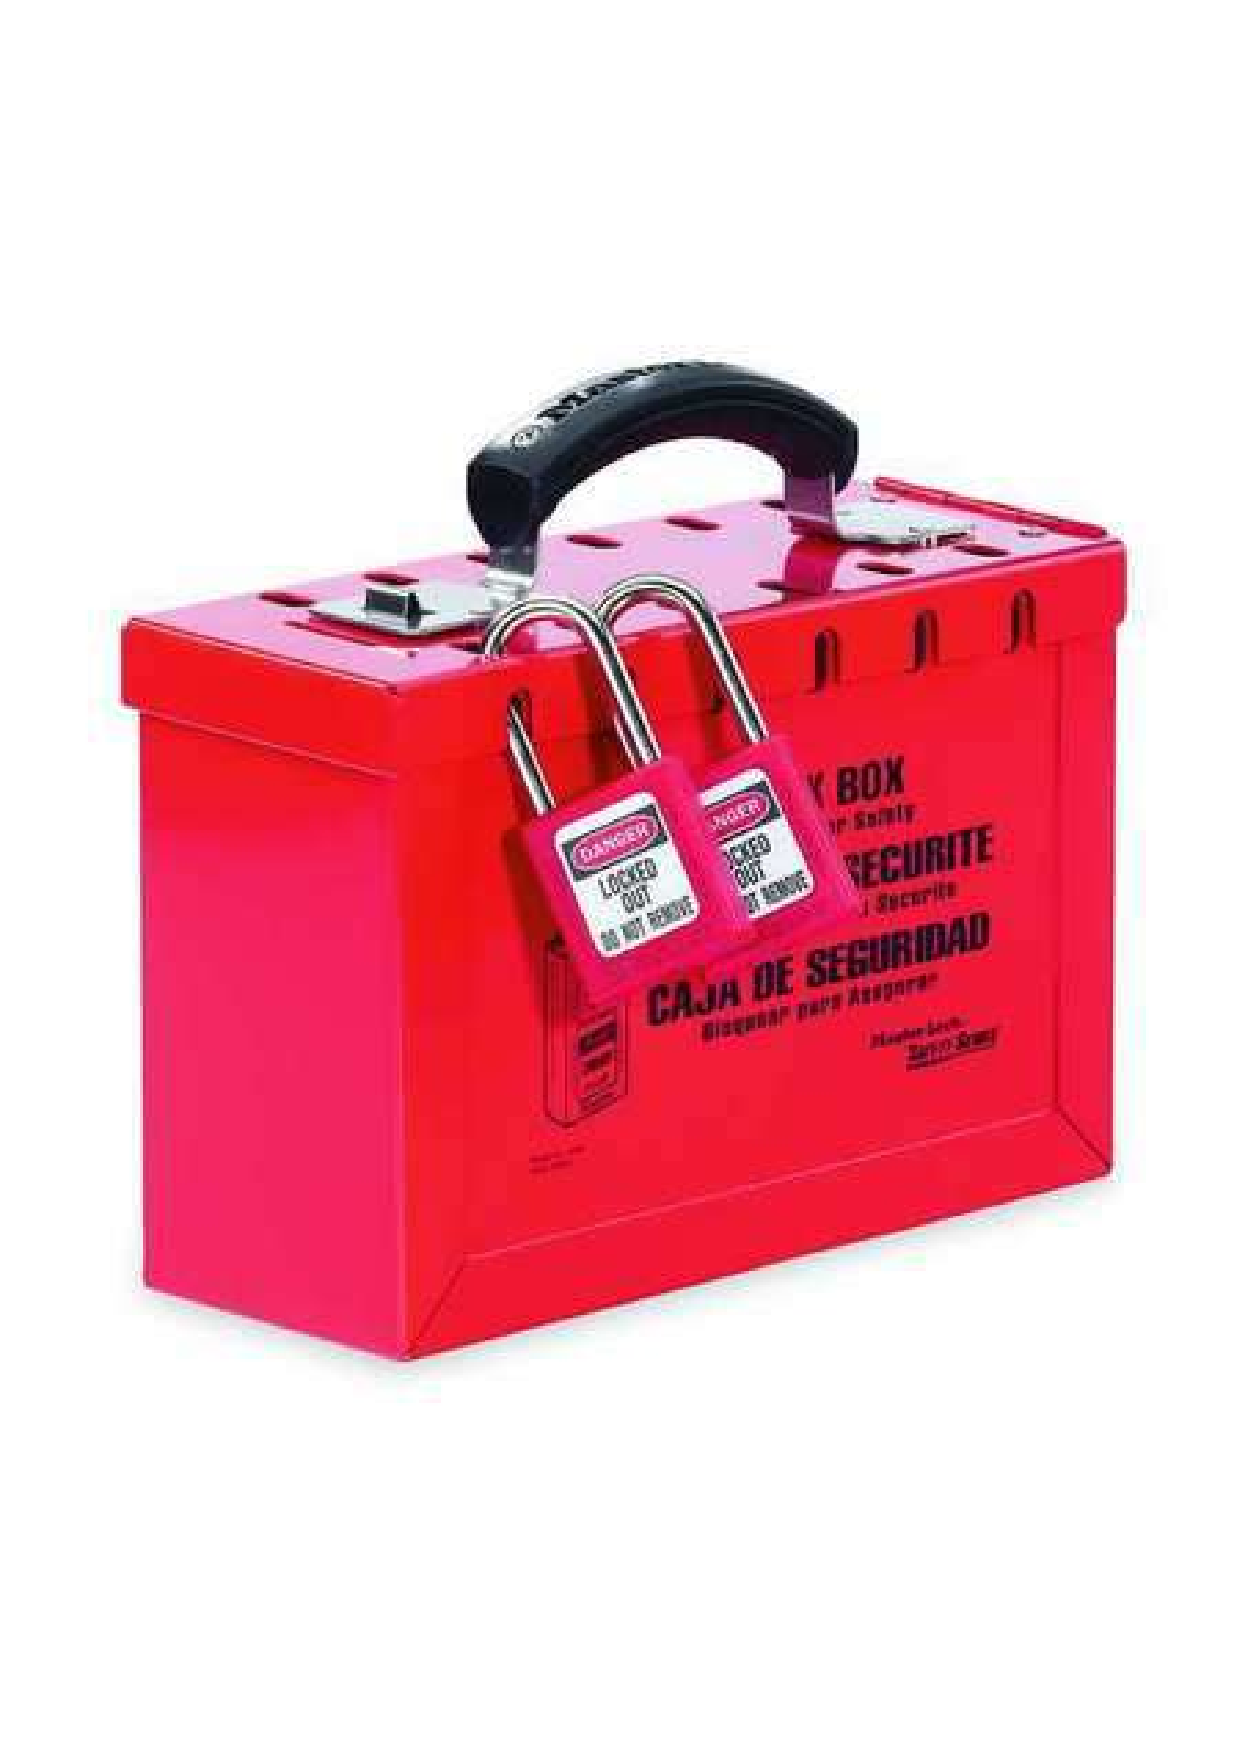
\includegraphics[scale=.35]{Z10BLufo5oy.pdf} 
\end{center}

\bigskip
\noindent
So let us talk about the physical solution: The solution entails Bob and Alice putting their own locks onto the box and then open their locks sequentially so that at each transfer the box will have some lock on it and there is no need for the key transfer. 

\bigskip
\noindent 
Now let us talk about the mathematical translation of this in information security:
Alice wants to send a message, which can be represented by $a$ mod $m$ to Bob (We assume that $GCD(a,m)=1$). So she chooses an exponent $e$ such that $GCD(e, \phi(m))=1$. Similarly Bob chooses his own exponent $d$ such that $GCD(d, \phi(m))=1$. Then both $e$ and $d$ have multiplicative inverses modulo $\phi(m)$. The exponents correspond to putting locks on the box, while the multiplicative inverse exponents correspond to unlocking.  Now, using Euler's congruence and Corollary 16, we see that the physical scheme we described above translates to the following mathematical proof:
$$(((a^e)^d)^{e^{-1}})^{d^{-1}} \equiv a^{1+k\phi(m)}\equiv a \pmod{m}.$$

\subsection{The RSA}
\begin{itemize}
    \item Designed by Rivest-Shamir-Adleman in 1978. 
    \item Is one of the first successful implementations of the new ``Public-key Cryptography" era
    \item Depends on Diffie-Helman key exchange
    \item Depends on the difficulty of factorization and large prime numbers
\end{itemize}

\bigskip
\noindent
{\bf The Scheme:} In this scheme there are two keys. One is called ``the Public Key" and the other called ``the Secret Key":
\\
{\bf Public Key:} For two large primes $p, q$ let $n=pq$. The public key is the ordered pair $(n,e)$ where $(e, \phi(n))=1$. 
\\
{\bf Secret Key:} $p, q$ and $d$ such that $d\equiv e^{-1} \pmod{\phi(n)}$.

\bigskip
\noindent
In RSA everybody can encrypt a message using the public key: If $m$ is the message (a number, such that $(m,n)=1$), the encryption is done by sending $m^e$ modulo $n$ to the server. The server then decrypts this message by calculating $(m^e)^d$ modulo $n$. Why does this work? 
The scheme works since 
$$(m^e)^d = m^{1+\phi(m)\cdot k} \equiv m \pmod{n}$$
by Euler's congruence theorem.

\bigskip
\hrule
\section{Order of Elements in moduli, Primitive Elements}
We start with recalling that $a^{\phi(n)} \equiv 1 \pmod{n}$ for $GCD(a,n)=1$. So for example we know that $2^6 \equiv 1 \pmod{7}$. But we also have $2^3\equiv 1 \pmod{7}$. So, sometimes we can have a smaller power that is equivalent to 1. 

On the other hand if we check the powers of 3, we see that the smallest power of 3 that is 1 modulo 7 is 6.

This leads to the following definition:
\begin{definition} ({\bf Order of an element}) Let $n>1$ be an integer and $a$ be such that $GCD(a,n)=1$. The order of $a$ modulo $n$, denoted by $ord_n(a)$ is defined to be the smallest positive power of $a$ that is equivalent to 1 modulo $n$. In other words, 
$$ord_n(a)=h \Leftrightarrow a^h \equiv 1 \pmod{n}, \:\:\: a^k\not \equiv 1 \pmod{n}, \:\:\:  1\leq k < h.$$
\end{definition}
\begin{example}
Based on our observations above, $ord_7(2)=3$ and $ord_7(3)=6$.
\end{example}

\bigskip
\noindent
Before getting some theoretical results about the order, let us see some observations:
\begin{observation}
\begin{enumerate}
    \item For any $n>1$, $ord_n(a)=1$ if and only if $a\equiv 1 \pmod{n}$.
    \item By Euler's Theorem, we know $ord_n(a) \leq \phi(n)$ for each $n:GCD(a,n)=1$.
    \end{enumerate}
\end{observation}
\begin{theorem}
Suppose $ord_n(a)=h$. Then $a^m\equiv 1 \pmod{n}$ if and only if $h|m$. In particular, $ord_n(a)|\phi(n)$ for all $n>1$ and $a: (a,n)=1$. 
\end{theorem}

\begin{remark}
We should remember that in any context that we are talking about $ord_n(a)$, we must assume that $GCD(a,n)=1$. Indeed if $a^q\equiv 1 \pmod {n}$ then we can write $a\cdot a^{q-1}-nk=1$, which, by Bezout's theorem, implies that $GCD(a,n)=1$. 
\end{remark}
Let us look at an example of finding the order in the light of the previous theorem:
\begin{example}
To find $ord_{18}(5)$ for example, using the previous thoerem, we know that $ord_{18}(5)|\phi(18)=6$. So we just need to check $5^2, 5^3$ modulo $18$. $5^2=25 \equiv 7 \pmod{18}$ and so $5^3 \equiv 35 \equiv 17 \pmod{18}$. This shows that $ord_{18}(5)\neq 1, 2$ or $3$, so we must have $ord_{18}(5)=6$.  
\end{example}

\bigskip
\noindent

The following theorem gives us one of the most useful properties related to the order:
\begin{theorem}
If $ord_n(a)=h$, then $\{1,a,a^2, \dots, a^{h-1}\}$ are all distinct modulo $n$.
\end{theorem}

\begin{corollary}
If $ord_n(a)=\phi(n)$, then $\{1,a, a^2, \dots, a^{\phi(n)-1}\}$ forms a $C.S.R.R.C$ modulo $n$. In other words, we have 
$$\{1,a, a^2, \dots, a^{\phi(n)-1}\} \equiv \Z_n^{\times} \pmod{n}.$$
\end{corollary}
\begin{example}
Let us see the examples of $3$ modulo 7 and $2$ modulo 13:
$$\{3^1, 3^2, 3^3, 3^4, 3^5, 3^6\} \equiv \{3, 2, 6, 4, 5, 1\} \pmod{7}$$ and
$$\{2^1, 2^2, 2^3, 2^4, 2^5, 2^6, 2^7, 2^8, 2^9, 2^{10}, 2^{11}, 2^{12}\} \equiv \{2, 4, 8, 3, 6, 12, 11, 9, 5, 10, 7, 1\} \pmod{13}.$$
\end{example}

\bigskip
\noindent
The following theorem gives us a useful tool for finding orders of exponents:
\begin{theorem}
If $ord_n(a)=h$, then $ord_n(a^k) = \frac{h}{GCD(h,k)}$.
\end{theorem}

\bigskip
\noindent
We have the following immediate corollary:
\begin{corollary}
If $ord_{n}(a)=h$, then $ord_n(a^k)=h$ if and only if $GCD(h,k)=1$. 
\end{corollary}

\bigskip
\noindent
\begin{definition}
Let $a\in \Z$ and $m>1$ be an integer such that $GCD(a,n)=1$. We say that $a$ is a {\it primitive element(root)} modulo $n$ if $ord_n(a)=\phi(n)$.
\end{definition}

\begin{example}
Based on what we have seen before, we know that $3$ is a primitive element modulo $7$ and $2$ is a primitive element modulo 11, but $2$ is not a primitive element modulo $7$.
\end{example}

\bigskip
\noindent
There are two main questions regarding primitive elements:
\begin{enumerate}
    \item For which $n>1$, does there exist a primitive element modulo $n$?
    \item If there is a primitive element modulo $n$, how many primitive elements are there?
\end{enumerate}

\begin{example}
To understand this question more, let us look at the example of 12 and 16:
\\ $\phi(12)=4$ and the numbers relatively prime to $12$ are $1, 5, 7$ and $11$, but 
$$1^2\equiv 5^2\equiv 7^2\equiv 11^2 \equiv 1 \pmod{12}$$ so there are no primitive elements modulo $12$.

Similarly, $1^2 \equiv 7^2 \equiv 9^2 \equiv 15^2 \equiv 1 \pmod{16}$, whereas $3^4 \equiv5^4\equiv 11^4 \equiv 13^4 \equiv 1 \pmod{16}$. Since $\phi(16)=8$, there are no primitive elements modulo $16$. 
\end{example}

\bigskip
\noindent
We start with the following theorem that will eliminate many numbers from having primitive elements:
\begin{theorem}\label{prim1}
Let $m\geq 1$ be any integer and let $a$ be any odd integer. Then we have
$$a^{2^m} \equiv 1 \pmod{2^{m+2}}.$$
\end{theorem}
\begin{corollary}
Since $\phi(2^{m+2})=2^{m+1}$, the previous theorem shows that there is no primitive element modulo $2^{m}$ for $m\geq 3$.
\end{corollary}

The following theorem helps eliminate a much bigger set of numbers:
\begin{theorem}\label{prim2}
If $n=mk$, where $m,k>2$ and $GCD(m,k)=1$, then there is no primitive element modulo $n$.
\end{theorem}

\bigskip
\noindent
As a corollary to Theorem \ref{prim1} and Theorem \ref{prim2}, we have the following result:
\begin{corollary}
If there is a primitive element modulo $n$ then $n$ must be $2$, $4$, $p^k$ or $2p^k$, where $p$ is an odd prime. 
\end{corollary}

It turns out that the result in the previous corollary is actually two sided, which is a theorem that we will give without a proof.
\begin{theorem}
There is a primitive element modulo $n$ if and only if $n$ is 2, 4, $p^k$ or $2p^k$, where $p$ is an odd prime. 
\end{theorem}

\bigskip
\noindent
Recall that if $a$ is a primitive element modulo $n$, then 
$$\{1, a, a^2, \dots, a^{\phi(n)-1}\} \equiv \Z_n^{\times} \pmod{n}.$$

In particular, if $p$ is prime, then 
$$\{1, a, a^2, \dots, a^{p-2}\} \equiv \{1,2, \dots, p-1\} \pmod{p}.$$

\bigskip
\noindent
\begin{theorem}
If there is a primitive element modulo $n$, then there are exactly $\phi(\phi(n))$ primitive elements modulo $n$.
\end{theorem}
\begin{proof}
If $a$ is a primitive element modulo $n$, then by Corollary 18, $a^d$ is also a primitive element if and only if $GCD(d, \phi(n))=1$.
\end{proof}
\begin{example}
Using the idea in the proof, we can now find all primitive elements modulo $13$. We saw before that $2$ is a primitive element modulo $13$. Since $\phi(13)=12$, the set of all primitive elements modulo $13$ are $\{2, 2^5, 2^7, 2^{11}\}$ which is equivalent to $\{2, 6, 11, 7\}. $
\end{example}

\end{document} 